\documentclass{beamer}
\usepackage{siunitx}
\usepackage{tfrupee}
\let\vec\mathbf
\mode<presentation>
\usepackage{amsmath}
\usepackage{amssymb}
%\usepackage{advdate}
\usepackage{adjustbox}
%\usepackage{subcaption}
\usepackage{enumitem}
\usepackage{multicol}
\usepackage{mathtools}
\usepackage{listings}
\usepackage{url}
\usetheme{Boadilla}
\usecolortheme{lily}
\setbeamertemplate{footline}
{
  \leavevmode%
  \hbox{%
  \begin{beamercolorbox}[wd=\paperwidth,ht=2.25ex,dp=1ex,right]{author in head/foot}%
    \insertframenumber{} / \inserttotalframenumber\hspace*{2ex} 
  \end{beamercolorbox}}%
  \vskip0pt%
}
\setbeamertemplate{navigation symbols}{}
\providecommand{\nCr}[2]{\,^{#1}C_{#2}} % nCr
\providecommand{\nPr}[2]{\,^{#1}P_{#2}} % nPr
\providecommand{\mbf}{\mathbf}
\providecommand{\pr}[1]{\ensuremath{\Pr\left(#1\right)}}
\providecommand{\qfunc}[1]{\ensuremath{Q\left(#1\right)}}
\providecommand{\sbrak}[1]{\ensuremath{{}\left[#1\right]}}
\providecommand{\lsbrak}[1]{\ensuremath{{}\left[#1\right.}}
\providecommand{\rsbrak}[1]{\ensuremath{{}\left.#1\right]}}
\providecommand{\brak}[1]{\ensuremath{\left(#1\right)}}
\providecommand{\lbrak}[1]{\ensuremath{\left(#1\right.}}
\providecommand{\rbrak}[1]{\ensuremath{\left.#1\right)}}
\providecommand{\cbrak}[1]{\ensuremath{\left\{#1\right\}}}
\providecommand{\lcbrak}[1]{\ensuremath{\left\{#1\right.}}
\providecommand{\rcbrak}[1]{\ensuremath{\left.#1\right\}}}
\theoremstyle{remark}
\newtheorem{rem}{Remark}
\newcommand{\sgn}{\mathop{\mathrm{sgn}}}

\providecommand{\res}[1]{\Res\displaylimits_{#1}} 
\providecommand{\norm}[1]{\left\lVert#1\right\rVert}
\providecommand{\mtx}[1]{\mathbf{#1}}
\providecommand{\abs}[1]{\left\vert#1\right\vert}
\providecommand{\fourier}{\overset{\mathcal{F}}{ \rightleftharpoons}}
%\providecommand{\hilbert}{\overset{\mathcal{H}}{ \rightleftharpoons}}
\providecommand{\system}{\overset{\mathcal{H}}{ \longleftrightarrow}}
	%\newcommand{\solution}[2]{\textbf{Solution:}{#1}}
%\newcommand{\solution}{\noindent \textbf{Solution: }}align
\providecommand{\dec}[2]{\ensuremath{\overset{#1}{\underset{#2}{\gtrless}}}}
\newcommand{\myvec}[1]{\ensuremath{\begin{pmatrix}#1\end{pmatrix}}}

\title{Matrices in Geometry - 5.8.35}
\author{EE25BTECH11037  Divyansh}
\date{Sept, 2025}

\begin{document}

\maketitle


\section{Problem}
\begin{frame}
\frametitle{Problem Statement}
Let C be any circle with center $\brak{0, \sqrt{2}}$. Prove that at most two rational points can be there on C.  \brak{\text{A rational point is a point both of whose coordinates are rational numbers}}.
\end{frame}

\section{Solution}
\begin{frame}{Solution}
   
The equation of the given circle C can be written as 
\begin{align}
    C: \norm{\vec{x}-\vec{O}}=r
\end{align}
where r is the radius of circle C and $\vec{O}=\myvec{0\\\sqrt{2}}$ is the center of the circle.\\
Let $\vec{P}$ be a rational point on the circle, then
\begin{align}
    \norm{\vec{P} - \vec{O}} = r
\end{align}
Upon squaring both sides,
\begin{align}
    \norm{\vec{P} - \vec{O}}^2 = r^2 \implies \vec{P}^{\top}\vec{P} - 2\vec{P}^{\top}\vec{O} + \vec{O}^{\top}\vec{O} = r^2
\end{align}
\end{frame}

\begin{frame}{Solution}
Substituting $\vec{P}=\myvec{x \\ y}$ and $\vec{O}=\myvec{0 \\ \sqrt{2}}$
\begin{align}
    \myvec{x & y}\myvec{x \\ y} - 2 \myvec{x&y}\myvec{0 \\ \sqrt{2}} + \myvec{0 & \sqrt{2}}\myvec{0 \\ \sqrt{2}} = r^2\\
    \implies x^2 + y^2 - 2\sqrt{2}y + 2=r^2
\end{align}
Rearranging the terms,
\begin{align}
    x^2 + y^2 -r^2 + 2=2\sqrt{2}y\\
    \vec{P} \in R^2 \implies x, y \in R \implies \text{LHS is rational}\\ \implies \text{RHS should be rational} 
    \implies y=0 \\
    \therefore x^2 = r^2 -2 \implies x = \pm \sqrt{r^2 - 2}: r>\sqrt{2}
\end{align}
\end{frame}

\begin{frame}{Solution}
We get the points 
\begin{align}
    \vec{P}=\myvec{\sqrt{r^2 - 2}\\0} \text{ OR } \vec{P} = \myvec{-\sqrt{r^2 - 2}\\0} : r^2 - 2 \text{ is a perfect square} 
\end{align}
This proves that at most two rational points can be present in C.\\
Let us try to show this using a graph with $r=\sqrt{6}$.
\begin{figure}[H]
    \centering
    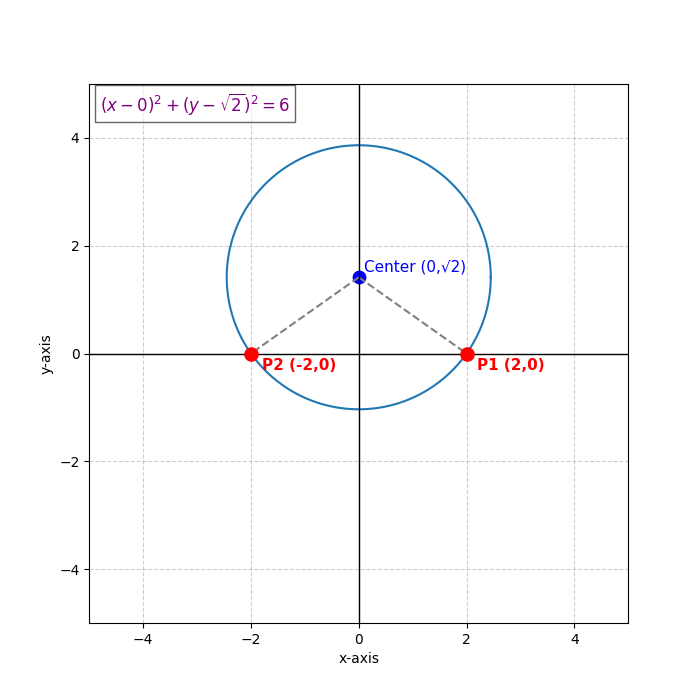
\includegraphics[width=0.4\columnwidth]{figs/1.png}
    \caption{Graph for 7.4.44 with $r= \sqrt{6}$}
    \label{fig:placeholder}
\end{figure}
\end{frame}


\end{document}
